\begin{frame}{Marking global inconsistencies?}
  Consider this program:
  \[%
    \ELam{f}{\TUnknown}{\EAp{f}{(\EPlus{f}{1})}}
  \]%

  \pause
  $\assignType{f}{\TUnknown}$, so the bidirectional system operates gradually, \pause
  but $f$ is 
  %
  \pause
  \begin{enumerate}
    \item applied as a function \pause (a function?)
      \pause
    \item an operand of $\ECOpPlus$ \pause (a number?)
  \end{enumerate}

  \pause
  \vspace{1em}
  \emph{Global, constraint-based type checking would have caught this!}

  \note[item]{Since the marked lambda calculus is for bidirectional systems, it might not do
    everything we'd like}
  \note[item]{In this program, the type of f is given to be unknown, so the bidirectional system
    would operate gradually}
  \note[item]{But we can notice that f is first of all applied as a function, so maybe it's a
    function?}
  \note[item]{But it's also on the left of plus, so maybe it's a number?}
  \note[item]{We think, well, some sort of global, constraint-based inference system would have
    caught this!}
\end{frame}

\begin{frame}{Layers upon layers}
  Get the best of both worlds by layering \textbf{constraint-based inference} 
  atop the marked lambda calculus \\[1em]

  \pause
  \begin{itemize}
    \item The marked lambda calculus localizes and recovers predictably from \emph{local inconsistencies}

      \pause
    \item \textbf{Type hole inference} solves and marks \emph{global inconsistencies}

      \pause
      \begin{itemize}
        \item Not meant to be a standalone type checker
        \item Downstream service to supplement the marked lambda calculus
      \end{itemize}
  \end{itemize}

  \note[item]{In the second part of this paper, we describe how we can the best of both worlds by
    layering a constraint-based inference system atop the marked lambda calculus}
  \note[item]{So the marked lambda calculus provides local inference with error localization and recovery}
  \note[item]{And the type hole inference, which would operate on the marked terms, solves and marks
    global inconsistencies like the one in the example}
  \note[item]{It's important to note that this isn't meant to be a standalone type checker, but
    rather a sort of downstream service to supplement the bidirectional system}
\end{frame}

\newcommand{\Id}[1]{\ensuremath{\goodcolor{hole}{#1}}}
\newcommand{\IdU}{\ensuremath{\Id{u}}}
\newcommand{\ProvU}{\ensuremath{\IdU}}
\newcommand{\ProvExp}[1]{\ensuremath{exp\goodcolor{\colorOkSideJudge}{(}#1\goodcolor{\colorOkSideJudge}{)}}}
\newcommand{\ProvIn}[1]{\ensuremath{\to_L\goodcolor{\colorOkSideJudge}{(}#1\goodcolor{\colorOkSideJudge}{)}}}
\newcommand{\ProvOut}[1]{\ensuremath{\to_R\goodcolor{\colorOkSideJudge}{(}#1\goodcolor{\colorOkSideJudge}{)}}}
\newcommand{\PTS}{\operatorname{\mathsf{PotentialTypeSet}}}
\newcommand{\cursor}{\ensuremath{\goodcolor{\colorOkSideJudge}{\bm{\wedge}}}}

\begin{frame}{Type hole inference}
  \begin{itemize}
    \item Occurrences of $\TUnknown$ arise from
      \pause (1) \emph{type holes}, \eg, in $\ELam{x}{\TUnknown}{\cdots}$ \\
      \pause or (2) error marks

      \pause
    \item Gather constraints from the bidirectional system\pause,
      treating occurrences of $\TUnknown$ as unification variables
      {\footnotesize\parencite{siek2008}}

      \pause
    \item Solve them via unification whilst maintaining partial solutions
      %
      \pause
      \begin{itemize}
        \item When solvable, proceeds as normal unification

          \pause
        \item When unsolvable, accumulates sets of all potential type \emph{fillings}, inferred from
          constraints, for each unknown type
      \end{itemize}
  \end{itemize}

  \note[item]{We observe that any occurrences of the unknown type arise from either these explicit
    annotations, which we call type holes because it's supposed that the programmer will eventually
    want to fill them in with some known type}
  \note[item]{We'll see how type hole inference facilitates this workflow}
  \note[item]{Or, the error marks that arise during marking}
  \note[item]{To describe type hole inference at a high level, we gather constraints bidirectionally
    from the marked syntax}
  \note[item]{and treat any occurrences of unknown as unification variables in the standard way}
  \note[item]{Then, we'll solve these constraints}
  \note[item]{and when they're solvable, we'll proceed as normal to find the substitution that can
    satisfy all the constraints}
  \note[item]{However, when there are inconsistent constraints, the system gracefully degrades to
    maintain partial solutions by accumulating the potential type fillings for each unknown type}
  \note[item]{Let's just see how this manifests in our implementation in Hazel---you can find the
    details of constraint generation and this solving process in the paper}
\end{frame}

\begin{frame}[fragile, t]
  \begin{center}
    \alt<2->{
      \alt<3->{
        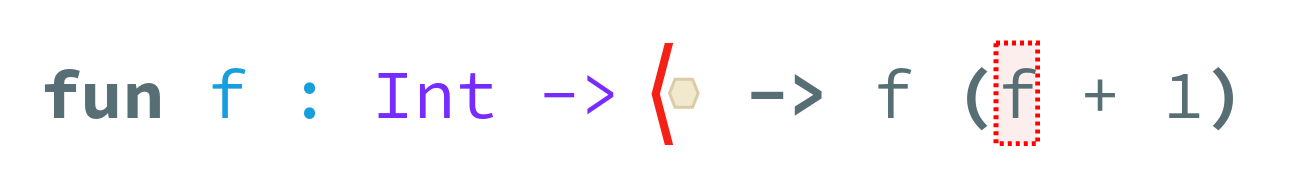
\includegraphics[width=0.9\textwidth]{inference-arrow.png}
      }{
        
\includegraphics[width=0.9\textwidth]{inference-int.png}
      }
    }{
      
\includegraphics[width=0.9\textwidth]{inference.png}
    }
    \vspace{2em}
    \alt<2->{
      \alt<3->{
        
\includegraphics[width=0.9\textwidth]{inspector-arrow.png}
      }{
        
\includegraphics[width=0.9\textwidth]{inspector-int.png}
      }
    }{
      
\includegraphics[width=0.9\textwidth]{inspector.png}
    }
  \end{center}

  \begin{center}
    \small
    Play around with this at
    \textcolor{MidnightBlue}{[\url{https://hazel.org/build/thi-old-engine-with-merge}]}
  \end{center}

  \begin{tikzpicture}[remember picture,overlay]
    \node[xshift=-4.6cm, yshift=-4.7cm, visible on=<2>] at (current page.north east) { \mousePointer };
    \node[xshift=-2.3cm, yshift=-4.7cm, visible on=<3>] at (current page.north east) { \mousePointer };
  \end{tikzpicture}

  \note[item]{Taking the same example from earlier into Hazel with type hole inference, we can see
    that when we hover onto the type hole, the cursor inspector tells us that there are conflicting
    constraints}
  \note[item]{which demand that f be an Int and an Int -> ? at the same time}
  \note[item]{because f is an operand of +, and it's being applied to the result of +}
  \note[item]{We have the option of selecting either one by clicking,}
  \note[item]{and by hovering over them, the code updates to show what would happen if we chose each
    one}
  \note[item]{When we hover over Int, it fills Int into the type hole, and now the application of f
    is marked with an error because control has, in some sense, been returned to the bidirectional
    system}
  \note[item]{Similarly, hovering over Int -> ? results in the second f being marked with an error}
\end{frame}

\begin{frame}
  This approach is \emph{neutral} \\[1em]

  \pause
  \begin{itemize}
    \item Localize errors to the originating type hole or error mark, \\
      instead of guessing about user intent

      \pause
    \item All potential type hole fillings are provided to the user for selection

      \pause
    \item Control returned to bidirectional system after user selects
  \end{itemize}

  \note[item]{This approach is neutral in the sense that we don't try to guess about user intent but
    simply provide all potential type hole fillings to the user for selection}
  \note[item]{facilitating a workflow of filling in type holes and returning control to the marked
    lambda calculus}
\end{frame}
